\documentclass{article}
\usepackage{tikz}
\begin{document}

% Prüferova sekvencia 1
\textbf{Strom č. 1}\\
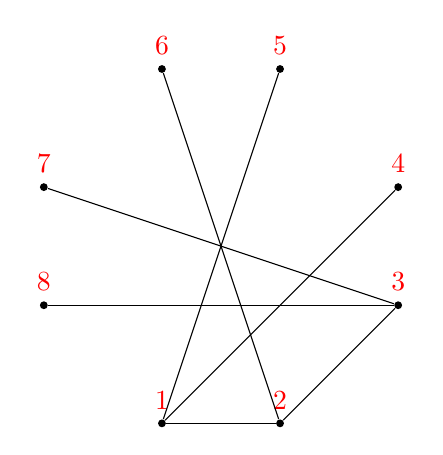
\begin{tikzpicture}[scale=1.5]
  \node[circle,fill=black,inner sep=1pt,label=above:{\textcolor{red}{1}}] (1) at (0,0) {};
  \node[circle,fill=black,inner sep=1pt,label=above:{\textcolor{red}{2}}] (2) at (1,0) {};
  \node[circle,fill=black,inner sep=1pt,label=above:{\textcolor{red}{3}}] (3) at (2,1) {};
  \node[circle,fill=black,inner sep=1pt,label=above:{\textcolor{red}{4}}] (4) at (2,2) {};
  \node[circle,fill=black,inner sep=1pt,label=above:{\textcolor{red}{5}}] (5) at (1,3) {};
  \node[circle,fill=black,inner sep=1pt,label=above:{\textcolor{red}{6}}] (6) at (0,3) {};
  \node[circle,fill=black,inner sep=1pt,label=above:{\textcolor{red}{7}}] (7) at (-1,2) {};
  \node[circle,fill=black,inner sep=1pt,label=above:{\textcolor{red}{8}}] (8) at (-1,1) {};
  \draw (4) -- (1);
  \draw (5) -- (1);
  \draw (1) -- (2);
  \draw (6) -- (2);
  \draw (2) -- (3);
  \draw (7) -- (3);
  \draw (3) -- (8);
\end{tikzpicture}

\vspace{2cm}

% Prüferova sekvencia 2
\textbf{Strom č. 2}\\
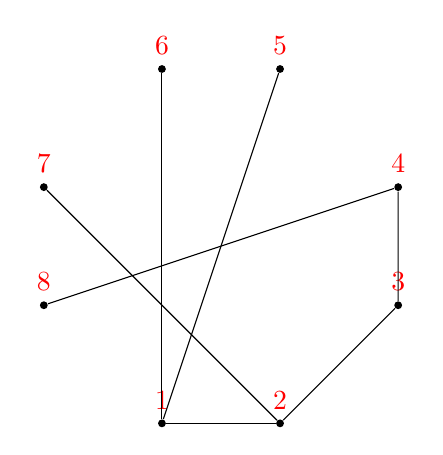
\begin{tikzpicture}[scale=1.5]
  \node[circle,fill=black,inner sep=1pt,label=above:{\textcolor{red}{1}}] (1) at (0,0) {};
  \node[circle,fill=black,inner sep=1pt,label=above:{\textcolor{red}{2}}] (2) at (1,0) {};
  \node[circle,fill=black,inner sep=1pt,label=above:{\textcolor{red}{3}}] (3) at (2,1) {};
  \node[circle,fill=black,inner sep=1pt,label=above:{\textcolor{red}{4}}] (4) at (2,2) {};
  \node[circle,fill=black,inner sep=1pt,label=above:{\textcolor{red}{5}}] (5) at (1,3) {};
  \node[circle,fill=black,inner sep=1pt,label=above:{\textcolor{red}{6}}] (6) at (0,3) {};
  \node[circle,fill=black,inner sep=1pt,label=above:{\textcolor{red}{7}}] (7) at (-1,2) {};
  \node[circle,fill=black,inner sep=1pt,label=above:{\textcolor{red}{8}}] (8) at (-1,1) {};
  \draw (5) -- (1);
  \draw (6) -- (1);
  \draw (1) -- (2);
  \draw (7) -- (2);
  \draw (2) -- (3);
  \draw (3) -- (4);
  \draw (4) -- (8);
\end{tikzpicture}

\vspace{2cm}

% Prüferova sekvencia 3
\textbf{Strom č. 3}\\
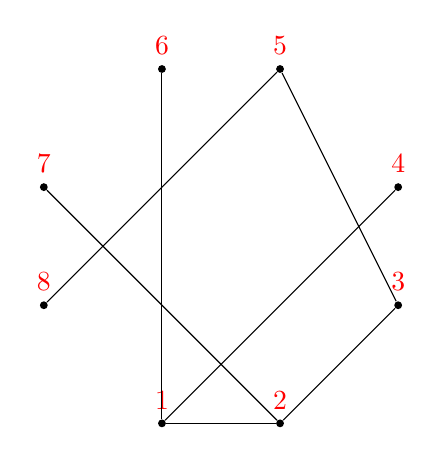
\begin{tikzpicture}[scale=1.5]
  \node[circle,fill=black,inner sep=1pt,label=above:{\textcolor{red}{1}}] (1) at (0,0) {};
  \node[circle,fill=black,inner sep=1pt,label=above:{\textcolor{red}{2}}] (2) at (1,0) {};
  \node[circle,fill=black,inner sep=1pt,label=above:{\textcolor{red}{3}}] (3) at (2,1) {};
  \node[circle,fill=black,inner sep=1pt,label=above:{\textcolor{red}{4}}] (4) at (2,2) {};
  \node[circle,fill=black,inner sep=1pt,label=above:{\textcolor{red}{5}}] (5) at (1,3) {};
  \node[circle,fill=black,inner sep=1pt,label=above:{\textcolor{red}{6}}] (6) at (0,3) {};
  \node[circle,fill=black,inner sep=1pt,label=above:{\textcolor{red}{7}}] (7) at (-1,2) {};
  \node[circle,fill=black,inner sep=1pt,label=above:{\textcolor{red}{8}}] (8) at (-1,1) {};
  \draw (4) -- (1);
  \draw (6) -- (1);
  \draw (1) -- (2);
  \draw (7) -- (2);
  \draw (2) -- (3);
  \draw (3) -- (5);
  \draw (5) -- (8);
\end{tikzpicture}

\vspace{2cm}

% Prüferova sekvencia 4
\textbf{Strom č. 4}\\
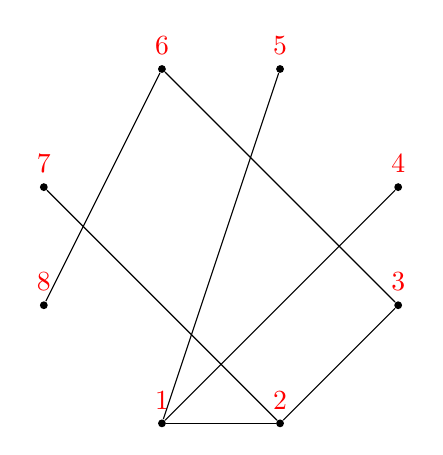
\begin{tikzpicture}[scale=1.5]
  \node[circle,fill=black,inner sep=1pt,label=above:{\textcolor{red}{1}}] (1) at (0,0) {};
  \node[circle,fill=black,inner sep=1pt,label=above:{\textcolor{red}{2}}] (2) at (1,0) {};
  \node[circle,fill=black,inner sep=1pt,label=above:{\textcolor{red}{3}}] (3) at (2,1) {};
  \node[circle,fill=black,inner sep=1pt,label=above:{\textcolor{red}{4}}] (4) at (2,2) {};
  \node[circle,fill=black,inner sep=1pt,label=above:{\textcolor{red}{5}}] (5) at (1,3) {};
  \node[circle,fill=black,inner sep=1pt,label=above:{\textcolor{red}{6}}] (6) at (0,3) {};
  \node[circle,fill=black,inner sep=1pt,label=above:{\textcolor{red}{7}}] (7) at (-1,2) {};
  \node[circle,fill=black,inner sep=1pt,label=above:{\textcolor{red}{8}}] (8) at (-1,1) {};
  \draw (4) -- (1);
  \draw (5) -- (1);
  \draw (1) -- (2);
  \draw (7) -- (2);
  \draw (2) -- (3);
  \draw (3) -- (6);
  \draw (6) -- (8);
\end{tikzpicture}

\vspace{2cm}

% Prüferova sekvencia 5
\textbf{Strom č. 5}\\
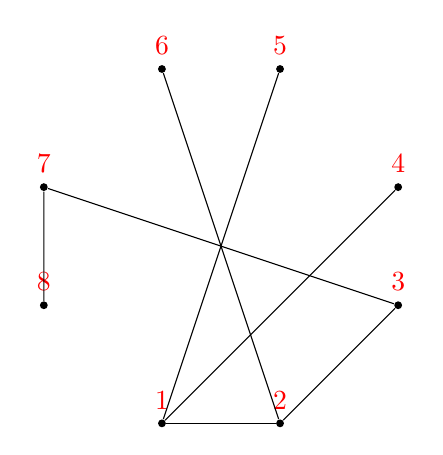
\begin{tikzpicture}[scale=1.5]
  \node[circle,fill=black,inner sep=1pt,label=above:{\textcolor{red}{1}}] (1) at (0,0) {};
  \node[circle,fill=black,inner sep=1pt,label=above:{\textcolor{red}{2}}] (2) at (1,0) {};
  \node[circle,fill=black,inner sep=1pt,label=above:{\textcolor{red}{3}}] (3) at (2,1) {};
  \node[circle,fill=black,inner sep=1pt,label=above:{\textcolor{red}{4}}] (4) at (2,2) {};
  \node[circle,fill=black,inner sep=1pt,label=above:{\textcolor{red}{5}}] (5) at (1,3) {};
  \node[circle,fill=black,inner sep=1pt,label=above:{\textcolor{red}{6}}] (6) at (0,3) {};
  \node[circle,fill=black,inner sep=1pt,label=above:{\textcolor{red}{7}}] (7) at (-1,2) {};
  \node[circle,fill=black,inner sep=1pt,label=above:{\textcolor{red}{8}}] (8) at (-1,1) {};
  \draw (4) -- (1);
  \draw (5) -- (1);
  \draw (1) -- (2);
  \draw (6) -- (2);
  \draw (2) -- (3);
  \draw (3) -- (7);
  \draw (7) -- (8);
\end{tikzpicture}

\vspace{2cm}

% Prüferova sekvencia 6
\textbf{Strom č. 6}\\
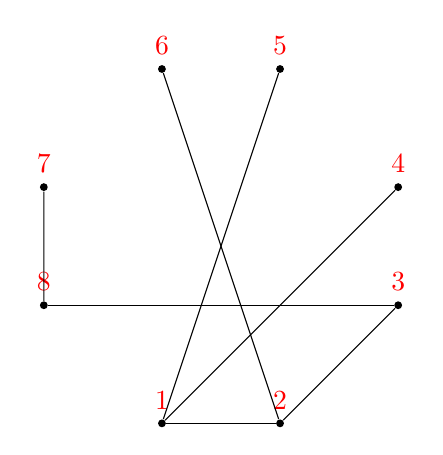
\begin{tikzpicture}[scale=1.5]
  \node[circle,fill=black,inner sep=1pt,label=above:{\textcolor{red}{1}}] (1) at (0,0) {};
  \node[circle,fill=black,inner sep=1pt,label=above:{\textcolor{red}{2}}] (2) at (1,0) {};
  \node[circle,fill=black,inner sep=1pt,label=above:{\textcolor{red}{3}}] (3) at (2,1) {};
  \node[circle,fill=black,inner sep=1pt,label=above:{\textcolor{red}{4}}] (4) at (2,2) {};
  \node[circle,fill=black,inner sep=1pt,label=above:{\textcolor{red}{5}}] (5) at (1,3) {};
  \node[circle,fill=black,inner sep=1pt,label=above:{\textcolor{red}{6}}] (6) at (0,3) {};
  \node[circle,fill=black,inner sep=1pt,label=above:{\textcolor{red}{7}}] (7) at (-1,2) {};
  \node[circle,fill=black,inner sep=1pt,label=above:{\textcolor{red}{8}}] (8) at (-1,1) {};
  \draw (4) -- (1);
  \draw (5) -- (1);
  \draw (1) -- (2);
  \draw (6) -- (2);
  \draw (2) -- (3);
  \draw (3) -- (8);
  \draw (7) -- (8);
\end{tikzpicture}

\vspace{2cm}

% Prüferova sekvencia 7
\textbf{Strom č. 7}\\
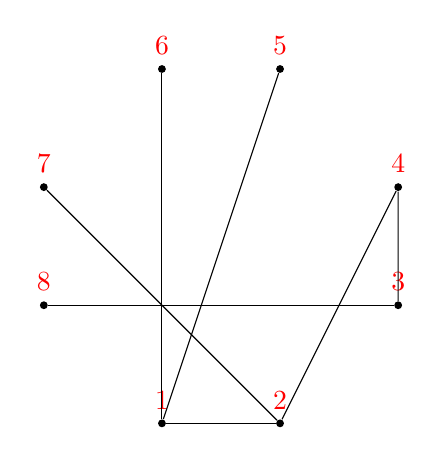
\begin{tikzpicture}[scale=1.5]
  \node[circle,fill=black,inner sep=1pt,label=above:{\textcolor{red}{1}}] (1) at (0,0) {};
  \node[circle,fill=black,inner sep=1pt,label=above:{\textcolor{red}{2}}] (2) at (1,0) {};
  \node[circle,fill=black,inner sep=1pt,label=above:{\textcolor{red}{3}}] (3) at (2,1) {};
  \node[circle,fill=black,inner sep=1pt,label=above:{\textcolor{red}{4}}] (4) at (2,2) {};
  \node[circle,fill=black,inner sep=1pt,label=above:{\textcolor{red}{5}}] (5) at (1,3) {};
  \node[circle,fill=black,inner sep=1pt,label=above:{\textcolor{red}{6}}] (6) at (0,3) {};
  \node[circle,fill=black,inner sep=1pt,label=above:{\textcolor{red}{7}}] (7) at (-1,2) {};
  \node[circle,fill=black,inner sep=1pt,label=above:{\textcolor{red}{8}}] (8) at (-1,1) {};
  \draw (5) -- (1);
  \draw (6) -- (1);
  \draw (1) -- (2);
  \draw (7) -- (2);
  \draw (2) -- (4);
  \draw (4) -- (3);
  \draw (3) -- (8);
\end{tikzpicture}

\vspace{2cm}

% Prüferova sekvencia 8
\textbf{Strom č. 8}\\
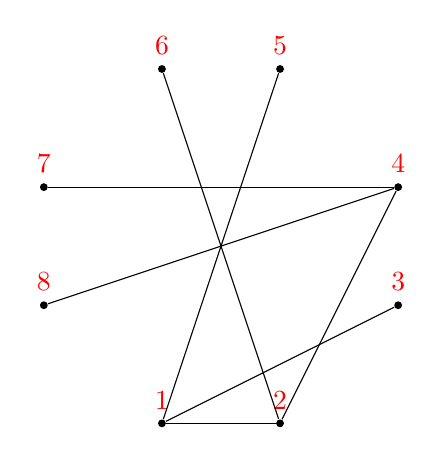
\begin{tikzpicture}[scale=1.5]
  \node[circle,fill=black,inner sep=1pt,label=above:{\textcolor{red}{1}}] (1) at (0,0) {};
  \node[circle,fill=black,inner sep=1pt,label=above:{\textcolor{red}{2}}] (2) at (1,0) {};
  \node[circle,fill=black,inner sep=1pt,label=above:{\textcolor{red}{3}}] (3) at (2,1) {};
  \node[circle,fill=black,inner sep=1pt,label=above:{\textcolor{red}{4}}] (4) at (2,2) {};
  \node[circle,fill=black,inner sep=1pt,label=above:{\textcolor{red}{5}}] (5) at (1,3) {};
  \node[circle,fill=black,inner sep=1pt,label=above:{\textcolor{red}{6}}] (6) at (0,3) {};
  \node[circle,fill=black,inner sep=1pt,label=above:{\textcolor{red}{7}}] (7) at (-1,2) {};
  \node[circle,fill=black,inner sep=1pt,label=above:{\textcolor{red}{8}}] (8) at (-1,1) {};
  \draw (3) -- (1);
  \draw (5) -- (1);
  \draw (1) -- (2);
  \draw (6) -- (2);
  \draw (2) -- (4);
  \draw (7) -- (4);
  \draw (4) -- (8);
\end{tikzpicture}

\vspace{2cm}

% Prüferova sekvencia 9
\textbf{Strom č. 9}\\
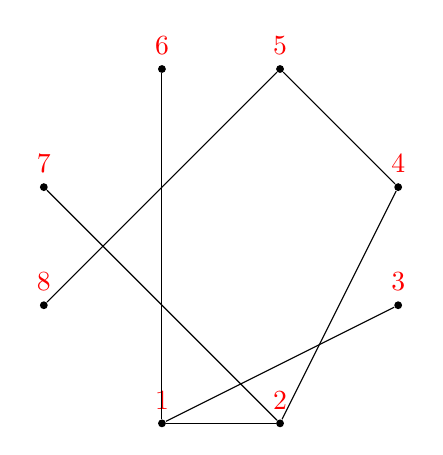
\begin{tikzpicture}[scale=1.5]
  \node[circle,fill=black,inner sep=1pt,label=above:{\textcolor{red}{1}}] (1) at (0,0) {};
  \node[circle,fill=black,inner sep=1pt,label=above:{\textcolor{red}{2}}] (2) at (1,0) {};
  \node[circle,fill=black,inner sep=1pt,label=above:{\textcolor{red}{3}}] (3) at (2,1) {};
  \node[circle,fill=black,inner sep=1pt,label=above:{\textcolor{red}{4}}] (4) at (2,2) {};
  \node[circle,fill=black,inner sep=1pt,label=above:{\textcolor{red}{5}}] (5) at (1,3) {};
  \node[circle,fill=black,inner sep=1pt,label=above:{\textcolor{red}{6}}] (6) at (0,3) {};
  \node[circle,fill=black,inner sep=1pt,label=above:{\textcolor{red}{7}}] (7) at (-1,2) {};
  \node[circle,fill=black,inner sep=1pt,label=above:{\textcolor{red}{8}}] (8) at (-1,1) {};
  \draw (3) -- (1);
  \draw (6) -- (1);
  \draw (1) -- (2);
  \draw (7) -- (2);
  \draw (2) -- (4);
  \draw (4) -- (5);
  \draw (5) -- (8);
\end{tikzpicture}

\vspace{2cm}

% Prüferova sekvencia 10
\textbf{Strom č. 10}\\
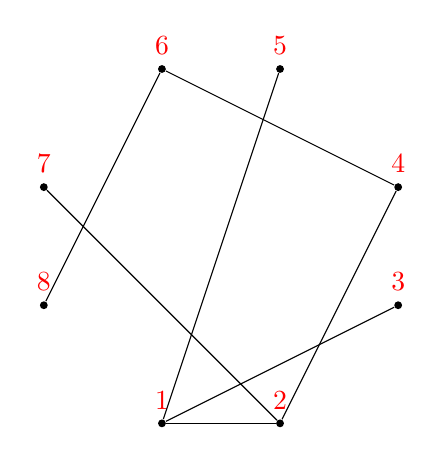
\begin{tikzpicture}[scale=1.5]
  \node[circle,fill=black,inner sep=1pt,label=above:{\textcolor{red}{1}}] (1) at (0,0) {};
  \node[circle,fill=black,inner sep=1pt,label=above:{\textcolor{red}{2}}] (2) at (1,0) {};
  \node[circle,fill=black,inner sep=1pt,label=above:{\textcolor{red}{3}}] (3) at (2,1) {};
  \node[circle,fill=black,inner sep=1pt,label=above:{\textcolor{red}{4}}] (4) at (2,2) {};
  \node[circle,fill=black,inner sep=1pt,label=above:{\textcolor{red}{5}}] (5) at (1,3) {};
  \node[circle,fill=black,inner sep=1pt,label=above:{\textcolor{red}{6}}] (6) at (0,3) {};
  \node[circle,fill=black,inner sep=1pt,label=above:{\textcolor{red}{7}}] (7) at (-1,2) {};
  \node[circle,fill=black,inner sep=1pt,label=above:{\textcolor{red}{8}}] (8) at (-1,1) {};
  \draw (3) -- (1);
  \draw (5) -- (1);
  \draw (1) -- (2);
  \draw (7) -- (2);
  \draw (2) -- (4);
  \draw (4) -- (6);
  \draw (6) -- (8);
\end{tikzpicture}

\vspace{2cm}

% Prüferova sekvencia 11
\textbf{Strom č. 11}\\
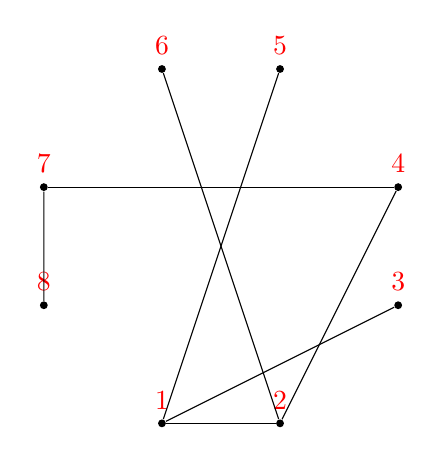
\begin{tikzpicture}[scale=1.5]
  \node[circle,fill=black,inner sep=1pt,label=above:{\textcolor{red}{1}}] (1) at (0,0) {};
  \node[circle,fill=black,inner sep=1pt,label=above:{\textcolor{red}{2}}] (2) at (1,0) {};
  \node[circle,fill=black,inner sep=1pt,label=above:{\textcolor{red}{3}}] (3) at (2,1) {};
  \node[circle,fill=black,inner sep=1pt,label=above:{\textcolor{red}{4}}] (4) at (2,2) {};
  \node[circle,fill=black,inner sep=1pt,label=above:{\textcolor{red}{5}}] (5) at (1,3) {};
  \node[circle,fill=black,inner sep=1pt,label=above:{\textcolor{red}{6}}] (6) at (0,3) {};
  \node[circle,fill=black,inner sep=1pt,label=above:{\textcolor{red}{7}}] (7) at (-1,2) {};
  \node[circle,fill=black,inner sep=1pt,label=above:{\textcolor{red}{8}}] (8) at (-1,1) {};
  \draw (3) -- (1);
  \draw (5) -- (1);
  \draw (1) -- (2);
  \draw (6) -- (2);
  \draw (2) -- (4);
  \draw (4) -- (7);
  \draw (7) -- (8);
\end{tikzpicture}

\vspace{2cm}

% Prüferova sekvencia 12
\textbf{Strom č. 12}\\
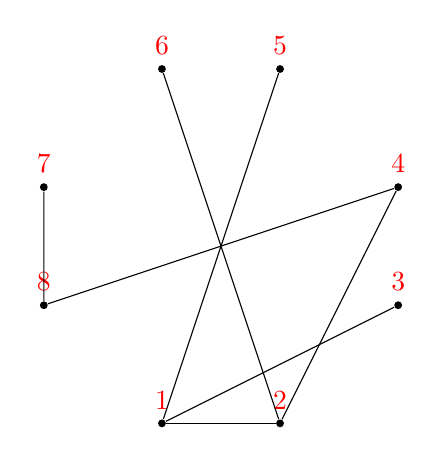
\begin{tikzpicture}[scale=1.5]
  \node[circle,fill=black,inner sep=1pt,label=above:{\textcolor{red}{1}}] (1) at (0,0) {};
  \node[circle,fill=black,inner sep=1pt,label=above:{\textcolor{red}{2}}] (2) at (1,0) {};
  \node[circle,fill=black,inner sep=1pt,label=above:{\textcolor{red}{3}}] (3) at (2,1) {};
  \node[circle,fill=black,inner sep=1pt,label=above:{\textcolor{red}{4}}] (4) at (2,2) {};
  \node[circle,fill=black,inner sep=1pt,label=above:{\textcolor{red}{5}}] (5) at (1,3) {};
  \node[circle,fill=black,inner sep=1pt,label=above:{\textcolor{red}{6}}] (6) at (0,3) {};
  \node[circle,fill=black,inner sep=1pt,label=above:{\textcolor{red}{7}}] (7) at (-1,2) {};
  \node[circle,fill=black,inner sep=1pt,label=above:{\textcolor{red}{8}}] (8) at (-1,1) {};
  \draw (3) -- (1);
  \draw (5) -- (1);
  \draw (1) -- (2);
  \draw (6) -- (2);
  \draw (2) -- (4);
  \draw (4) -- (8);
  \draw (7) -- (8);
\end{tikzpicture}

\vspace{2cm}

% Prüferova sekvencia 13
\textbf{Strom č. 13}\\
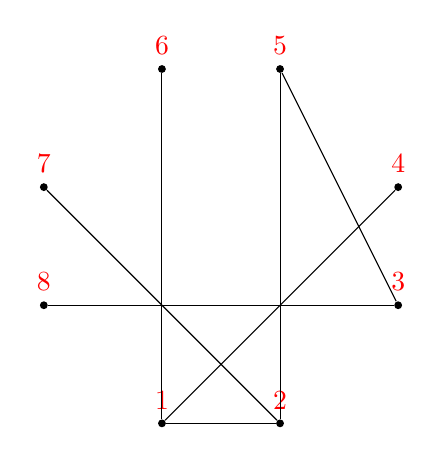
\begin{tikzpicture}[scale=1.5]
  \node[circle,fill=black,inner sep=1pt,label=above:{\textcolor{red}{1}}] (1) at (0,0) {};
  \node[circle,fill=black,inner sep=1pt,label=above:{\textcolor{red}{2}}] (2) at (1,0) {};
  \node[circle,fill=black,inner sep=1pt,label=above:{\textcolor{red}{3}}] (3) at (2,1) {};
  \node[circle,fill=black,inner sep=1pt,label=above:{\textcolor{red}{4}}] (4) at (2,2) {};
  \node[circle,fill=black,inner sep=1pt,label=above:{\textcolor{red}{5}}] (5) at (1,3) {};
  \node[circle,fill=black,inner sep=1pt,label=above:{\textcolor{red}{6}}] (6) at (0,3) {};
  \node[circle,fill=black,inner sep=1pt,label=above:{\textcolor{red}{7}}] (7) at (-1,2) {};
  \node[circle,fill=black,inner sep=1pt,label=above:{\textcolor{red}{8}}] (8) at (-1,1) {};
  \draw (4) -- (1);
  \draw (6) -- (1);
  \draw (1) -- (2);
  \draw (7) -- (2);
  \draw (2) -- (5);
  \draw (5) -- (3);
  \draw (3) -- (8);
\end{tikzpicture}

\vspace{2cm}

% Prüferova sekvencia 14
\textbf{Strom č. 14}\\
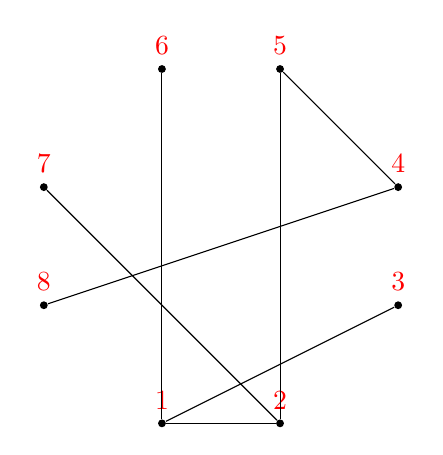
\begin{tikzpicture}[scale=1.5]
  \node[circle,fill=black,inner sep=1pt,label=above:{\textcolor{red}{1}}] (1) at (0,0) {};
  \node[circle,fill=black,inner sep=1pt,label=above:{\textcolor{red}{2}}] (2) at (1,0) {};
  \node[circle,fill=black,inner sep=1pt,label=above:{\textcolor{red}{3}}] (3) at (2,1) {};
  \node[circle,fill=black,inner sep=1pt,label=above:{\textcolor{red}{4}}] (4) at (2,2) {};
  \node[circle,fill=black,inner sep=1pt,label=above:{\textcolor{red}{5}}] (5) at (1,3) {};
  \node[circle,fill=black,inner sep=1pt,label=above:{\textcolor{red}{6}}] (6) at (0,3) {};
  \node[circle,fill=black,inner sep=1pt,label=above:{\textcolor{red}{7}}] (7) at (-1,2) {};
  \node[circle,fill=black,inner sep=1pt,label=above:{\textcolor{red}{8}}] (8) at (-1,1) {};
  \draw (3) -- (1);
  \draw (6) -- (1);
  \draw (1) -- (2);
  \draw (7) -- (2);
  \draw (2) -- (5);
  \draw (5) -- (4);
  \draw (4) -- (8);
\end{tikzpicture}

\vspace{2cm}

% Prüferova sekvencia 15
\textbf{Strom č. 15}\\
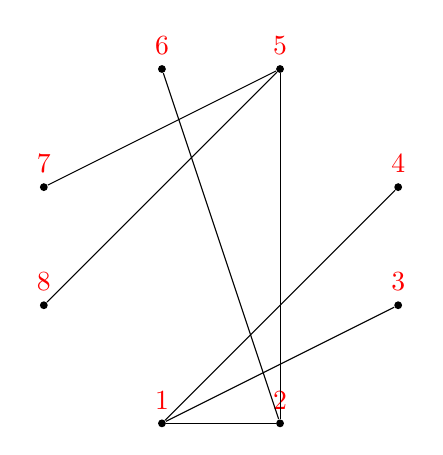
\begin{tikzpicture}[scale=1.5]
  \node[circle,fill=black,inner sep=1pt,label=above:{\textcolor{red}{1}}] (1) at (0,0) {};
  \node[circle,fill=black,inner sep=1pt,label=above:{\textcolor{red}{2}}] (2) at (1,0) {};
  \node[circle,fill=black,inner sep=1pt,label=above:{\textcolor{red}{3}}] (3) at (2,1) {};
  \node[circle,fill=black,inner sep=1pt,label=above:{\textcolor{red}{4}}] (4) at (2,2) {};
  \node[circle,fill=black,inner sep=1pt,label=above:{\textcolor{red}{5}}] (5) at (1,3) {};
  \node[circle,fill=black,inner sep=1pt,label=above:{\textcolor{red}{6}}] (6) at (0,3) {};
  \node[circle,fill=black,inner sep=1pt,label=above:{\textcolor{red}{7}}] (7) at (-1,2) {};
  \node[circle,fill=black,inner sep=1pt,label=above:{\textcolor{red}{8}}] (8) at (-1,1) {};
  \draw (3) -- (1);
  \draw (4) -- (1);
  \draw (1) -- (2);
  \draw (6) -- (2);
  \draw (2) -- (5);
  \draw (7) -- (5);
  \draw (5) -- (8);
\end{tikzpicture}

\vspace{2cm}

% Prüferova sekvencia 16
\textbf{Strom č. 16}\\
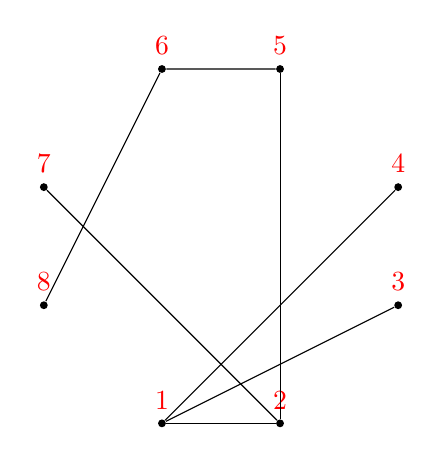
\begin{tikzpicture}[scale=1.5]
  \node[circle,fill=black,inner sep=1pt,label=above:{\textcolor{red}{1}}] (1) at (0,0) {};
  \node[circle,fill=black,inner sep=1pt,label=above:{\textcolor{red}{2}}] (2) at (1,0) {};
  \node[circle,fill=black,inner sep=1pt,label=above:{\textcolor{red}{3}}] (3) at (2,1) {};
  \node[circle,fill=black,inner sep=1pt,label=above:{\textcolor{red}{4}}] (4) at (2,2) {};
  \node[circle,fill=black,inner sep=1pt,label=above:{\textcolor{red}{5}}] (5) at (1,3) {};
  \node[circle,fill=black,inner sep=1pt,label=above:{\textcolor{red}{6}}] (6) at (0,3) {};
  \node[circle,fill=black,inner sep=1pt,label=above:{\textcolor{red}{7}}] (7) at (-1,2) {};
  \node[circle,fill=black,inner sep=1pt,label=above:{\textcolor{red}{8}}] (8) at (-1,1) {};
  \draw (3) -- (1);
  \draw (4) -- (1);
  \draw (1) -- (2);
  \draw (7) -- (2);
  \draw (2) -- (5);
  \draw (5) -- (6);
  \draw (6) -- (8);
\end{tikzpicture}

\vspace{2cm}

% Prüferova sekvencia 17
\textbf{Strom č. 17}\\
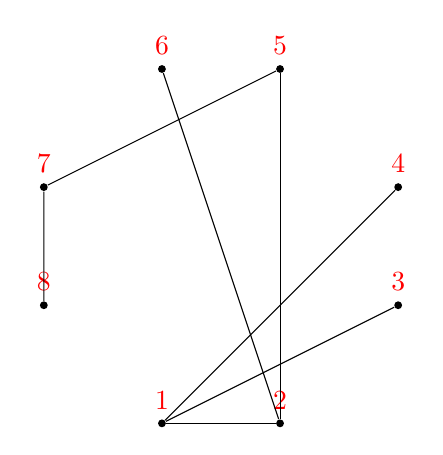
\begin{tikzpicture}[scale=1.5]
  \node[circle,fill=black,inner sep=1pt,label=above:{\textcolor{red}{1}}] (1) at (0,0) {};
  \node[circle,fill=black,inner sep=1pt,label=above:{\textcolor{red}{2}}] (2) at (1,0) {};
  \node[circle,fill=black,inner sep=1pt,label=above:{\textcolor{red}{3}}] (3) at (2,1) {};
  \node[circle,fill=black,inner sep=1pt,label=above:{\textcolor{red}{4}}] (4) at (2,2) {};
  \node[circle,fill=black,inner sep=1pt,label=above:{\textcolor{red}{5}}] (5) at (1,3) {};
  \node[circle,fill=black,inner sep=1pt,label=above:{\textcolor{red}{6}}] (6) at (0,3) {};
  \node[circle,fill=black,inner sep=1pt,label=above:{\textcolor{red}{7}}] (7) at (-1,2) {};
  \node[circle,fill=black,inner sep=1pt,label=above:{\textcolor{red}{8}}] (8) at (-1,1) {};
  \draw (3) -- (1);
  \draw (4) -- (1);
  \draw (1) -- (2);
  \draw (6) -- (2);
  \draw (2) -- (5);
  \draw (5) -- (7);
  \draw (7) -- (8);
\end{tikzpicture}

\vspace{2cm}

% Prüferova sekvencia 18
\textbf{Strom č. 18}\\
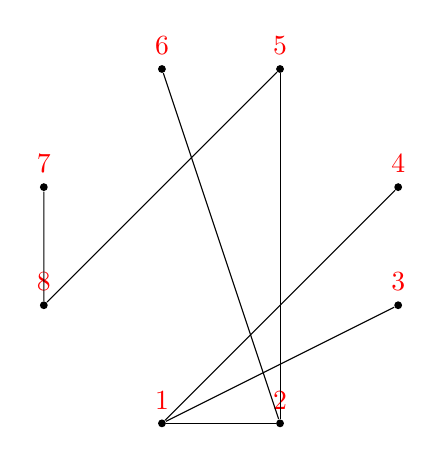
\begin{tikzpicture}[scale=1.5]
  \node[circle,fill=black,inner sep=1pt,label=above:{\textcolor{red}{1}}] (1) at (0,0) {};
  \node[circle,fill=black,inner sep=1pt,label=above:{\textcolor{red}{2}}] (2) at (1,0) {};
  \node[circle,fill=black,inner sep=1pt,label=above:{\textcolor{red}{3}}] (3) at (2,1) {};
  \node[circle,fill=black,inner sep=1pt,label=above:{\textcolor{red}{4}}] (4) at (2,2) {};
  \node[circle,fill=black,inner sep=1pt,label=above:{\textcolor{red}{5}}] (5) at (1,3) {};
  \node[circle,fill=black,inner sep=1pt,label=above:{\textcolor{red}{6}}] (6) at (0,3) {};
  \node[circle,fill=black,inner sep=1pt,label=above:{\textcolor{red}{7}}] (7) at (-1,2) {};
  \node[circle,fill=black,inner sep=1pt,label=above:{\textcolor{red}{8}}] (8) at (-1,1) {};
  \draw (3) -- (1);
  \draw (4) -- (1);
  \draw (1) -- (2);
  \draw (6) -- (2);
  \draw (2) -- (5);
  \draw (5) -- (8);
  \draw (7) -- (8);
\end{tikzpicture}

\vspace{2cm}

% Prüferova sekvencia 19
\textbf{Strom č. 19}\\
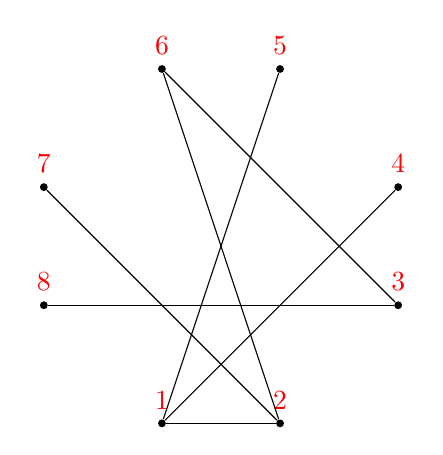
\begin{tikzpicture}[scale=1.5]
  \node[circle,fill=black,inner sep=1pt,label=above:{\textcolor{red}{1}}] (1) at (0,0) {};
  \node[circle,fill=black,inner sep=1pt,label=above:{\textcolor{red}{2}}] (2) at (1,0) {};
  \node[circle,fill=black,inner sep=1pt,label=above:{\textcolor{red}{3}}] (3) at (2,1) {};
  \node[circle,fill=black,inner sep=1pt,label=above:{\textcolor{red}{4}}] (4) at (2,2) {};
  \node[circle,fill=black,inner sep=1pt,label=above:{\textcolor{red}{5}}] (5) at (1,3) {};
  \node[circle,fill=black,inner sep=1pt,label=above:{\textcolor{red}{6}}] (6) at (0,3) {};
  \node[circle,fill=black,inner sep=1pt,label=above:{\textcolor{red}{7}}] (7) at (-1,2) {};
  \node[circle,fill=black,inner sep=1pt,label=above:{\textcolor{red}{8}}] (8) at (-1,1) {};
  \draw (4) -- (1);
  \draw (5) -- (1);
  \draw (1) -- (2);
  \draw (7) -- (2);
  \draw (2) -- (6);
  \draw (6) -- (3);
  \draw (3) -- (8);
\end{tikzpicture}

\vspace{2cm}

% Prüferova sekvencia 20
\textbf{Strom č. 20}\\
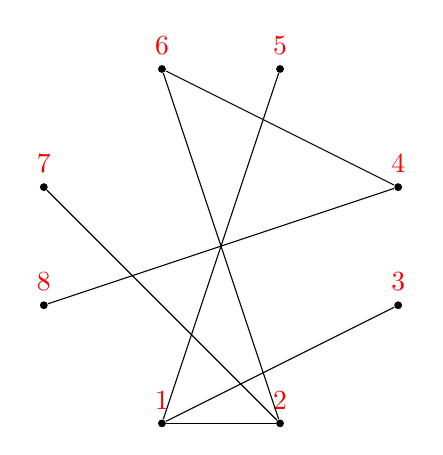
\begin{tikzpicture}[scale=1.5]
  \node[circle,fill=black,inner sep=1pt,label=above:{\textcolor{red}{1}}] (1) at (0,0) {};
  \node[circle,fill=black,inner sep=1pt,label=above:{\textcolor{red}{2}}] (2) at (1,0) {};
  \node[circle,fill=black,inner sep=1pt,label=above:{\textcolor{red}{3}}] (3) at (2,1) {};
  \node[circle,fill=black,inner sep=1pt,label=above:{\textcolor{red}{4}}] (4) at (2,2) {};
  \node[circle,fill=black,inner sep=1pt,label=above:{\textcolor{red}{5}}] (5) at (1,3) {};
  \node[circle,fill=black,inner sep=1pt,label=above:{\textcolor{red}{6}}] (6) at (0,3) {};
  \node[circle,fill=black,inner sep=1pt,label=above:{\textcolor{red}{7}}] (7) at (-1,2) {};
  \node[circle,fill=black,inner sep=1pt,label=above:{\textcolor{red}{8}}] (8) at (-1,1) {};
  \draw (3) -- (1);
  \draw (5) -- (1);
  \draw (1) -- (2);
  \draw (7) -- (2);
  \draw (2) -- (6);
  \draw (6) -- (4);
  \draw (4) -- (8);
\end{tikzpicture}

\vspace{2cm}

% Prüferova sekvencia 21
\textbf{Strom č. 21}\\
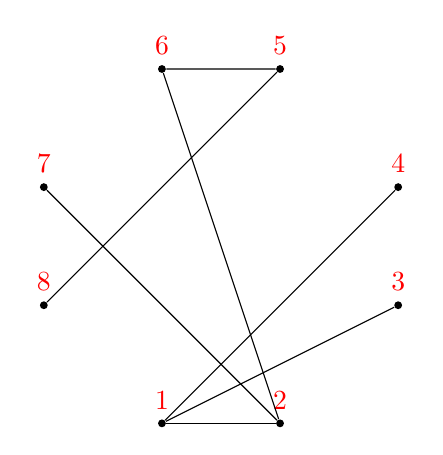
\begin{tikzpicture}[scale=1.5]
  \node[circle,fill=black,inner sep=1pt,label=above:{\textcolor{red}{1}}] (1) at (0,0) {};
  \node[circle,fill=black,inner sep=1pt,label=above:{\textcolor{red}{2}}] (2) at (1,0) {};
  \node[circle,fill=black,inner sep=1pt,label=above:{\textcolor{red}{3}}] (3) at (2,1) {};
  \node[circle,fill=black,inner sep=1pt,label=above:{\textcolor{red}{4}}] (4) at (2,2) {};
  \node[circle,fill=black,inner sep=1pt,label=above:{\textcolor{red}{5}}] (5) at (1,3) {};
  \node[circle,fill=black,inner sep=1pt,label=above:{\textcolor{red}{6}}] (6) at (0,3) {};
  \node[circle,fill=black,inner sep=1pt,label=above:{\textcolor{red}{7}}] (7) at (-1,2) {};
  \node[circle,fill=black,inner sep=1pt,label=above:{\textcolor{red}{8}}] (8) at (-1,1) {};
  \draw (3) -- (1);
  \draw (4) -- (1);
  \draw (1) -- (2);
  \draw (7) -- (2);
  \draw (2) -- (6);
  \draw (6) -- (5);
  \draw (5) -- (8);
\end{tikzpicture}

\vspace{2cm}

% Prüferova sekvencia 22
\textbf{Strom č. 22}\\
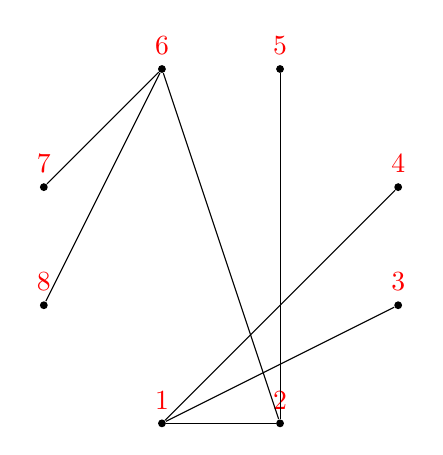
\begin{tikzpicture}[scale=1.5]
  \node[circle,fill=black,inner sep=1pt,label=above:{\textcolor{red}{1}}] (1) at (0,0) {};
  \node[circle,fill=black,inner sep=1pt,label=above:{\textcolor{red}{2}}] (2) at (1,0) {};
  \node[circle,fill=black,inner sep=1pt,label=above:{\textcolor{red}{3}}] (3) at (2,1) {};
  \node[circle,fill=black,inner sep=1pt,label=above:{\textcolor{red}{4}}] (4) at (2,2) {};
  \node[circle,fill=black,inner sep=1pt,label=above:{\textcolor{red}{5}}] (5) at (1,3) {};
  \node[circle,fill=black,inner sep=1pt,label=above:{\textcolor{red}{6}}] (6) at (0,3) {};
  \node[circle,fill=black,inner sep=1pt,label=above:{\textcolor{red}{7}}] (7) at (-1,2) {};
  \node[circle,fill=black,inner sep=1pt,label=above:{\textcolor{red}{8}}] (8) at (-1,1) {};
  \draw (3) -- (1);
  \draw (4) -- (1);
  \draw (1) -- (2);
  \draw (5) -- (2);
  \draw (2) -- (6);
  \draw (7) -- (6);
  \draw (6) -- (8);
\end{tikzpicture}

\vspace{2cm}

% Prüferova sekvencia 23
\textbf{Strom č. 23}\\
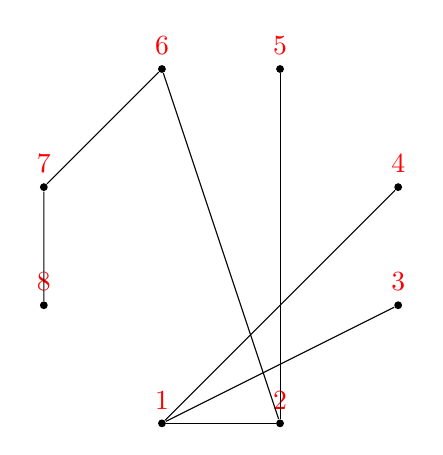
\begin{tikzpicture}[scale=1.5]
  \node[circle,fill=black,inner sep=1pt,label=above:{\textcolor{red}{1}}] (1) at (0,0) {};
  \node[circle,fill=black,inner sep=1pt,label=above:{\textcolor{red}{2}}] (2) at (1,0) {};
  \node[circle,fill=black,inner sep=1pt,label=above:{\textcolor{red}{3}}] (3) at (2,1) {};
  \node[circle,fill=black,inner sep=1pt,label=above:{\textcolor{red}{4}}] (4) at (2,2) {};
  \node[circle,fill=black,inner sep=1pt,label=above:{\textcolor{red}{5}}] (5) at (1,3) {};
  \node[circle,fill=black,inner sep=1pt,label=above:{\textcolor{red}{6}}] (6) at (0,3) {};
  \node[circle,fill=black,inner sep=1pt,label=above:{\textcolor{red}{7}}] (7) at (-1,2) {};
  \node[circle,fill=black,inner sep=1pt,label=above:{\textcolor{red}{8}}] (8) at (-1,1) {};
  \draw (3) -- (1);
  \draw (4) -- (1);
  \draw (1) -- (2);
  \draw (5) -- (2);
  \draw (2) -- (6);
  \draw (6) -- (7);
  \draw (7) -- (8);
\end{tikzpicture}

\vspace{2cm}

% Prüferova sekvencia 24
\textbf{Strom č. 24}\\
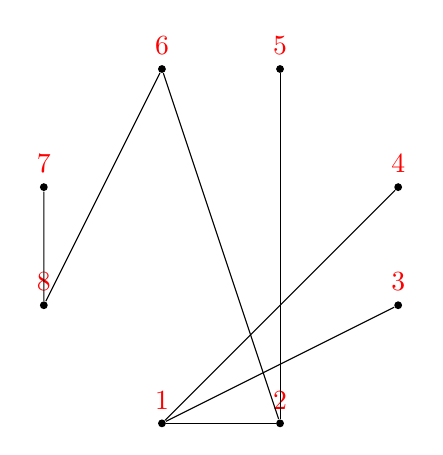
\begin{tikzpicture}[scale=1.5]
  \node[circle,fill=black,inner sep=1pt,label=above:{\textcolor{red}{1}}] (1) at (0,0) {};
  \node[circle,fill=black,inner sep=1pt,label=above:{\textcolor{red}{2}}] (2) at (1,0) {};
  \node[circle,fill=black,inner sep=1pt,label=above:{\textcolor{red}{3}}] (3) at (2,1) {};
  \node[circle,fill=black,inner sep=1pt,label=above:{\textcolor{red}{4}}] (4) at (2,2) {};
  \node[circle,fill=black,inner sep=1pt,label=above:{\textcolor{red}{5}}] (5) at (1,3) {};
  \node[circle,fill=black,inner sep=1pt,label=above:{\textcolor{red}{6}}] (6) at (0,3) {};
  \node[circle,fill=black,inner sep=1pt,label=above:{\textcolor{red}{7}}] (7) at (-1,2) {};
  \node[circle,fill=black,inner sep=1pt,label=above:{\textcolor{red}{8}}] (8) at (-1,1) {};
  \draw (3) -- (1);
  \draw (4) -- (1);
  \draw (1) -- (2);
  \draw (5) -- (2);
  \draw (2) -- (6);
  \draw (6) -- (8);
  \draw (7) -- (8);
\end{tikzpicture}

\vspace{2cm}

% Prüferova sekvencia 25
\textbf{Strom č. 25}\\
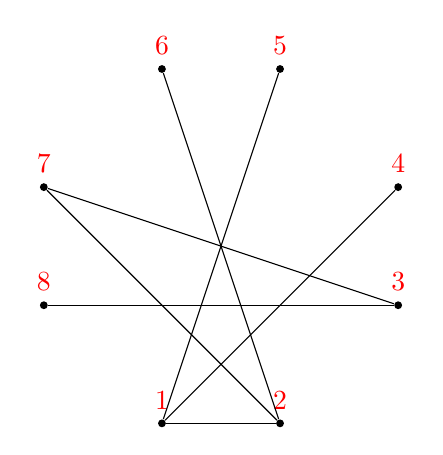
\begin{tikzpicture}[scale=1.5]
  \node[circle,fill=black,inner sep=1pt,label=above:{\textcolor{red}{1}}] (1) at (0,0) {};
  \node[circle,fill=black,inner sep=1pt,label=above:{\textcolor{red}{2}}] (2) at (1,0) {};
  \node[circle,fill=black,inner sep=1pt,label=above:{\textcolor{red}{3}}] (3) at (2,1) {};
  \node[circle,fill=black,inner sep=1pt,label=above:{\textcolor{red}{4}}] (4) at (2,2) {};
  \node[circle,fill=black,inner sep=1pt,label=above:{\textcolor{red}{5}}] (5) at (1,3) {};
  \node[circle,fill=black,inner sep=1pt,label=above:{\textcolor{red}{6}}] (6) at (0,3) {};
  \node[circle,fill=black,inner sep=1pt,label=above:{\textcolor{red}{7}}] (7) at (-1,2) {};
  \node[circle,fill=black,inner sep=1pt,label=above:{\textcolor{red}{8}}] (8) at (-1,1) {};
  \draw (4) -- (1);
  \draw (5) -- (1);
  \draw (1) -- (2);
  \draw (6) -- (2);
  \draw (2) -- (7);
  \draw (7) -- (3);
  \draw (3) -- (8);
\end{tikzpicture}

\vspace{2cm}

% Prüferova sekvencia 26
\textbf{Strom č. 26}\\
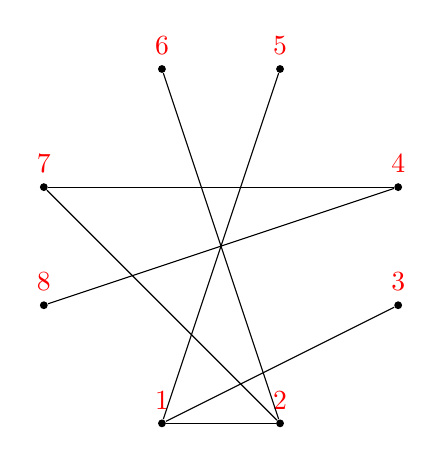
\begin{tikzpicture}[scale=1.5]
  \node[circle,fill=black,inner sep=1pt,label=above:{\textcolor{red}{1}}] (1) at (0,0) {};
  \node[circle,fill=black,inner sep=1pt,label=above:{\textcolor{red}{2}}] (2) at (1,0) {};
  \node[circle,fill=black,inner sep=1pt,label=above:{\textcolor{red}{3}}] (3) at (2,1) {};
  \node[circle,fill=black,inner sep=1pt,label=above:{\textcolor{red}{4}}] (4) at (2,2) {};
  \node[circle,fill=black,inner sep=1pt,label=above:{\textcolor{red}{5}}] (5) at (1,3) {};
  \node[circle,fill=black,inner sep=1pt,label=above:{\textcolor{red}{6}}] (6) at (0,3) {};
  \node[circle,fill=black,inner sep=1pt,label=above:{\textcolor{red}{7}}] (7) at (-1,2) {};
  \node[circle,fill=black,inner sep=1pt,label=above:{\textcolor{red}{8}}] (8) at (-1,1) {};
  \draw (3) -- (1);
  \draw (5) -- (1);
  \draw (1) -- (2);
  \draw (6) -- (2);
  \draw (2) -- (7);
  \draw (7) -- (4);
  \draw (4) -- (8);
\end{tikzpicture}

\vspace{2cm}

% Prüferova sekvencia 27
\textbf{Strom č. 27}\\
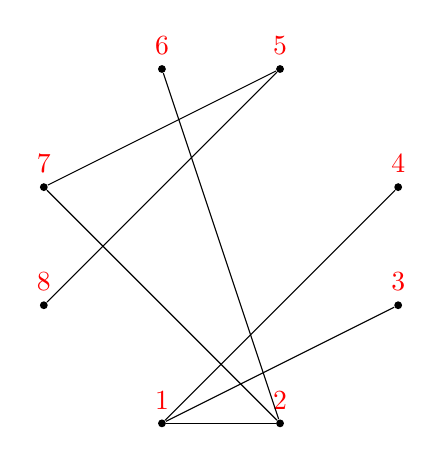
\begin{tikzpicture}[scale=1.5]
  \node[circle,fill=black,inner sep=1pt,label=above:{\textcolor{red}{1}}] (1) at (0,0) {};
  \node[circle,fill=black,inner sep=1pt,label=above:{\textcolor{red}{2}}] (2) at (1,0) {};
  \node[circle,fill=black,inner sep=1pt,label=above:{\textcolor{red}{3}}] (3) at (2,1) {};
  \node[circle,fill=black,inner sep=1pt,label=above:{\textcolor{red}{4}}] (4) at (2,2) {};
  \node[circle,fill=black,inner sep=1pt,label=above:{\textcolor{red}{5}}] (5) at (1,3) {};
  \node[circle,fill=black,inner sep=1pt,label=above:{\textcolor{red}{6}}] (6) at (0,3) {};
  \node[circle,fill=black,inner sep=1pt,label=above:{\textcolor{red}{7}}] (7) at (-1,2) {};
  \node[circle,fill=black,inner sep=1pt,label=above:{\textcolor{red}{8}}] (8) at (-1,1) {};
  \draw (3) -- (1);
  \draw (4) -- (1);
  \draw (1) -- (2);
  \draw (6) -- (2);
  \draw (2) -- (7);
  \draw (7) -- (5);
  \draw (5) -- (8);
\end{tikzpicture}

\vspace{2cm}

% Prüferova sekvencia 28
\textbf{Strom č. 28}\\
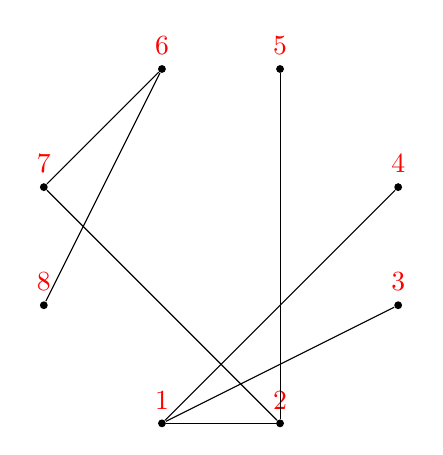
\begin{tikzpicture}[scale=1.5]
  \node[circle,fill=black,inner sep=1pt,label=above:{\textcolor{red}{1}}] (1) at (0,0) {};
  \node[circle,fill=black,inner sep=1pt,label=above:{\textcolor{red}{2}}] (2) at (1,0) {};
  \node[circle,fill=black,inner sep=1pt,label=above:{\textcolor{red}{3}}] (3) at (2,1) {};
  \node[circle,fill=black,inner sep=1pt,label=above:{\textcolor{red}{4}}] (4) at (2,2) {};
  \node[circle,fill=black,inner sep=1pt,label=above:{\textcolor{red}{5}}] (5) at (1,3) {};
  \node[circle,fill=black,inner sep=1pt,label=above:{\textcolor{red}{6}}] (6) at (0,3) {};
  \node[circle,fill=black,inner sep=1pt,label=above:{\textcolor{red}{7}}] (7) at (-1,2) {};
  \node[circle,fill=black,inner sep=1pt,label=above:{\textcolor{red}{8}}] (8) at (-1,1) {};
  \draw (3) -- (1);
  \draw (4) -- (1);
  \draw (1) -- (2);
  \draw (5) -- (2);
  \draw (2) -- (7);
  \draw (7) -- (6);
  \draw (6) -- (8);
\end{tikzpicture}

\vspace{2cm}

% Prüferova sekvencia 29
\textbf{Strom č. 29}\\
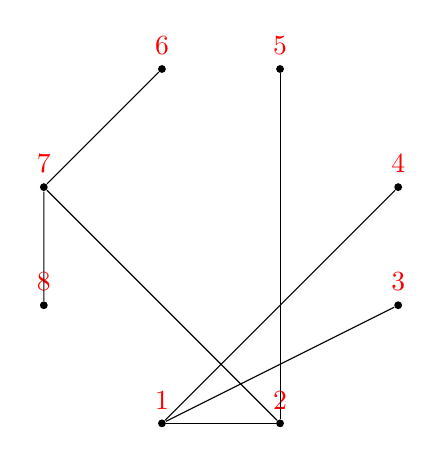
\begin{tikzpicture}[scale=1.5]
  \node[circle,fill=black,inner sep=1pt,label=above:{\textcolor{red}{1}}] (1) at (0,0) {};
  \node[circle,fill=black,inner sep=1pt,label=above:{\textcolor{red}{2}}] (2) at (1,0) {};
  \node[circle,fill=black,inner sep=1pt,label=above:{\textcolor{red}{3}}] (3) at (2,1) {};
  \node[circle,fill=black,inner sep=1pt,label=above:{\textcolor{red}{4}}] (4) at (2,2) {};
  \node[circle,fill=black,inner sep=1pt,label=above:{\textcolor{red}{5}}] (5) at (1,3) {};
  \node[circle,fill=black,inner sep=1pt,label=above:{\textcolor{red}{6}}] (6) at (0,3) {};
  \node[circle,fill=black,inner sep=1pt,label=above:{\textcolor{red}{7}}] (7) at (-1,2) {};
  \node[circle,fill=black,inner sep=1pt,label=above:{\textcolor{red}{8}}] (8) at (-1,1) {};
  \draw (3) -- (1);
  \draw (4) -- (1);
  \draw (1) -- (2);
  \draw (5) -- (2);
  \draw (2) -- (7);
  \draw (6) -- (7);
  \draw (7) -- (8);
\end{tikzpicture}

\vspace{2cm}

% Prüferova sekvencia 30
\textbf{Strom č. 30}\\
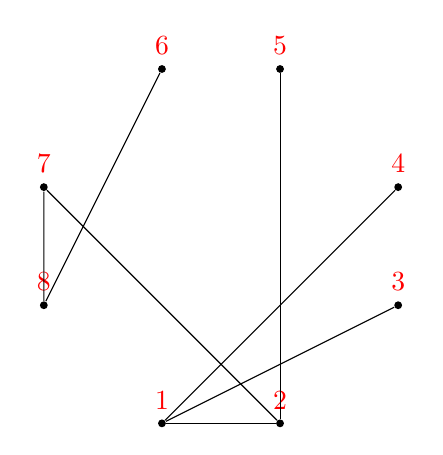
\begin{tikzpicture}[scale=1.5]
  \node[circle,fill=black,inner sep=1pt,label=above:{\textcolor{red}{1}}] (1) at (0,0) {};
  \node[circle,fill=black,inner sep=1pt,label=above:{\textcolor{red}{2}}] (2) at (1,0) {};
  \node[circle,fill=black,inner sep=1pt,label=above:{\textcolor{red}{3}}] (3) at (2,1) {};
  \node[circle,fill=black,inner sep=1pt,label=above:{\textcolor{red}{4}}] (4) at (2,2) {};
  \node[circle,fill=black,inner sep=1pt,label=above:{\textcolor{red}{5}}] (5) at (1,3) {};
  \node[circle,fill=black,inner sep=1pt,label=above:{\textcolor{red}{6}}] (6) at (0,3) {};
  \node[circle,fill=black,inner sep=1pt,label=above:{\textcolor{red}{7}}] (7) at (-1,2) {};
  \node[circle,fill=black,inner sep=1pt,label=above:{\textcolor{red}{8}}] (8) at (-1,1) {};
  \draw (3) -- (1);
  \draw (4) -- (1);
  \draw (1) -- (2);
  \draw (5) -- (2);
  \draw (2) -- (7);
  \draw (6) -- (8);
  \draw (7) -- (8);
\end{tikzpicture}

\vspace{2cm}

\end{document}
